%!TEX root = ../thesis.tex
% ******************************* Thesis Appendix A ****************************
\chapter{Supplementary information for Chapter \ref{ch4:title}} 

\section{ESMs included in the analysis of pothole cooling anomaly by \citet{zhangRoleAnthropogenicAerosols2021}}

\begin{small}
\begin{longtable}{>{\raggedright}p{3.25cm} >{\raggedright}p{3.25cm} >{\raggedright}p{3.5cm} >{\raggedright\arraybackslash}p{3.5cm}}
    \caption[Information of models included in the study by \citet{zhangRoleAnthropogenicAerosols2021}]{Information of models included in the study by \citet{zhangRoleAnthropogenicAerosols2021}}
    \label{tab:zhang-model}
    \\
    \toprule
     Model developer (Model) & Tropospheric chemistry model & Sulfur chemistry scheme & Aerosol scheme \\
     \midrule
     \endfirsthead

    \toprule
     Model developer (Model) & Tropospheric chemistry model & Sulfur chemistry scheme & Aerosol scheme \\
     \midrule
     \endhead
     
     \bottomrule
     \endlastfoot

     
     Met Office’s Hadley Centre for Climate Prediction and Research; MOHC (UKESM1-0-LL) Ref. \citet{sellarUKESM1DescriptionEvaluation2019,archibaldDescriptionEvaluationUKCA2020,mulcahyDescriptionEvaluationAerosol2020}  & UKCA (United Kingdom Chemistry and Aerosol) model with unified stratospheric-tropospheric chemistry (StratTrop) & Prognostic oxidant fields. Prognostic sulfur chemistry. & Aerosol scheme GLOMAP-mode. Two-moment, five size modes. 4 species: sulfate (\ce{SO4}), black carbon (BC), organic matter (OM) and sea salt. \\
     \midrule
     Norwegian Climate Center; NCC (NorESM2-LM). Ref. \citet{kirkevagProductiontaggedAerosolModule2018, selandOverviewNorwegianEarth2020} & Atmosphere model component CAM6-Nor built improvements on the CAM6 version from CESM2.1 & Diagnostic tropospheric oxidant fields: OH, \ce{O3}, \ce{H2O2}.  Prognostic  sulfur chemistry & 4 aerosol modes. 6 species: SOA, BC, \ce{SO4}, OM, Seasalt, and dust.  \\ 
     \midrule
     Max Planck Institute for Meteorology; MPI (MPI-ESM-1-2-HAM) Ref. \citet{neubauerGlobalAerosolClimate2019,neubauerHAMMOZConsortiumMPIESM12HAM2019,tegenGlobalAerosolClimate2019} & Atmospheric Model Component ECHAM6.3. &  Diagnostic oxidant fields: OH, \ce{H2O2}, \ce{NO2}, \ce{O3}, and \ce{NO3}. Prognostic sulfur chemistry. & Aerosol scheme HAM2.3. Two-moment. 7 modes: 4 soluble and 3 insoluble \\
     \midrule
     US Department of Commerce/ NOAA/Geophysical Fluid Dynamics Laboratory; GFDL (GFDL-ESM4) Ref. \citet{zhaoGFDLGlobalAtmosphere2018, heldStructurePerformanceGFDL2019, dunneGFDLEarthSystem2020} & Atmospheric component AM4.1 & Prognostic oxidant fields: OH, \ce{O3}, \ce{H2O2}, \ce{NO3}. Prognostic sulfur chemistry. & 5 aerosol types: sulfate, dust, black carbon, organic carbon, and sea salt.  \\
     \midrule
     European consortium of meteorological services, research institutes, and high-performance computing centers (EC-Earth-AerChem) Ref. \citet{vannoijeECEarth3AerChemGlobalClimate2021} & Aerosols and atmospheric chemistry are simulated with the Tracer Model version 5 (TM5), specifically release 3.0 of the massively parallel version of TM5 (TM5-mp 3.0). & The model includes aqueous-phase reactions for the oxidation of total dissolved sulfur dioxide & Modal aerosol microphysical scheme M7. 5 aerosol types: \ce{SO4}, BC, OA, sea salt, and mineral dust. 7 modes: 4 water-soluble and 3 insoluble modes  \\
     \midrule
     Beijing Climate Center; BCC (BCC-ESM1) Ref. \citet{zhangBCCESM1ModelDatasets2021} &  Atmospheric component is BCCAGCM3-Chem based on MOZART2 & Prognostic oxidant fields. Prognostic sulfur chemistry. & 5 aerosol species: \ce{SO4}, OC, BC, soil dust, and sea salt \\


\end{longtable}
\end{small}


\section{Supplementary figures}
\begin{figure}
    \centering
    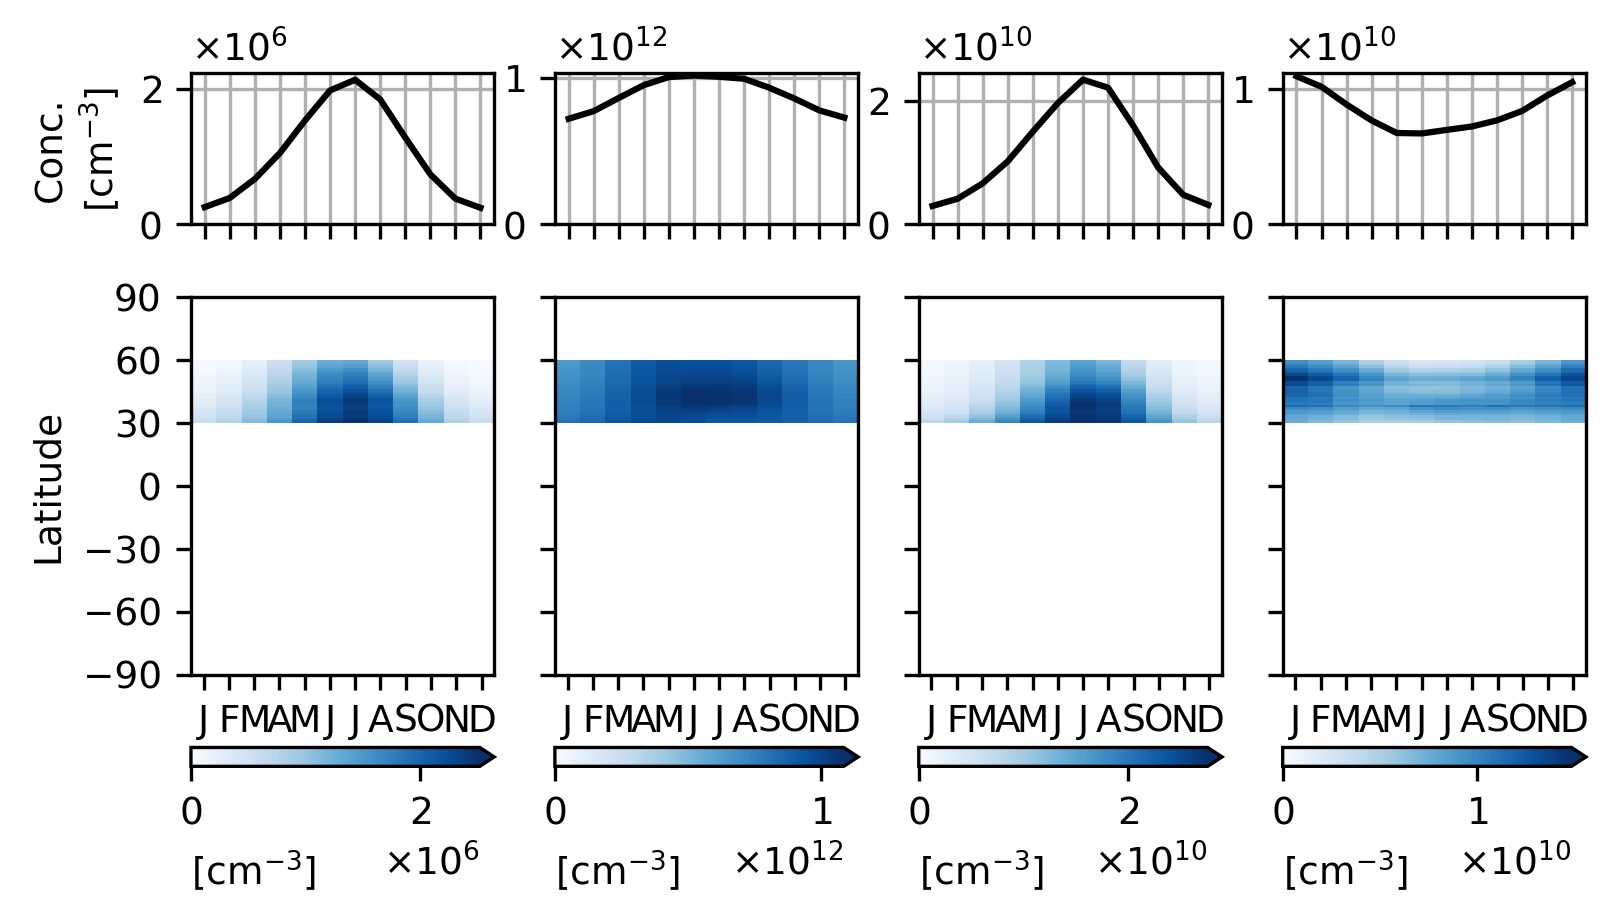
\includegraphics{Appendix1/figs/seasonal_oxidant_1980_lat30-60.png}
    \caption{Mean oxidant concentration between 1980 and 1989 from the surface up to 5 km and latitude 30 to 60\textdegree N }
    \label{fig:app1:seasonal-oxidant-30-60}
\end{figure}

\begin{figure}
    \centering
    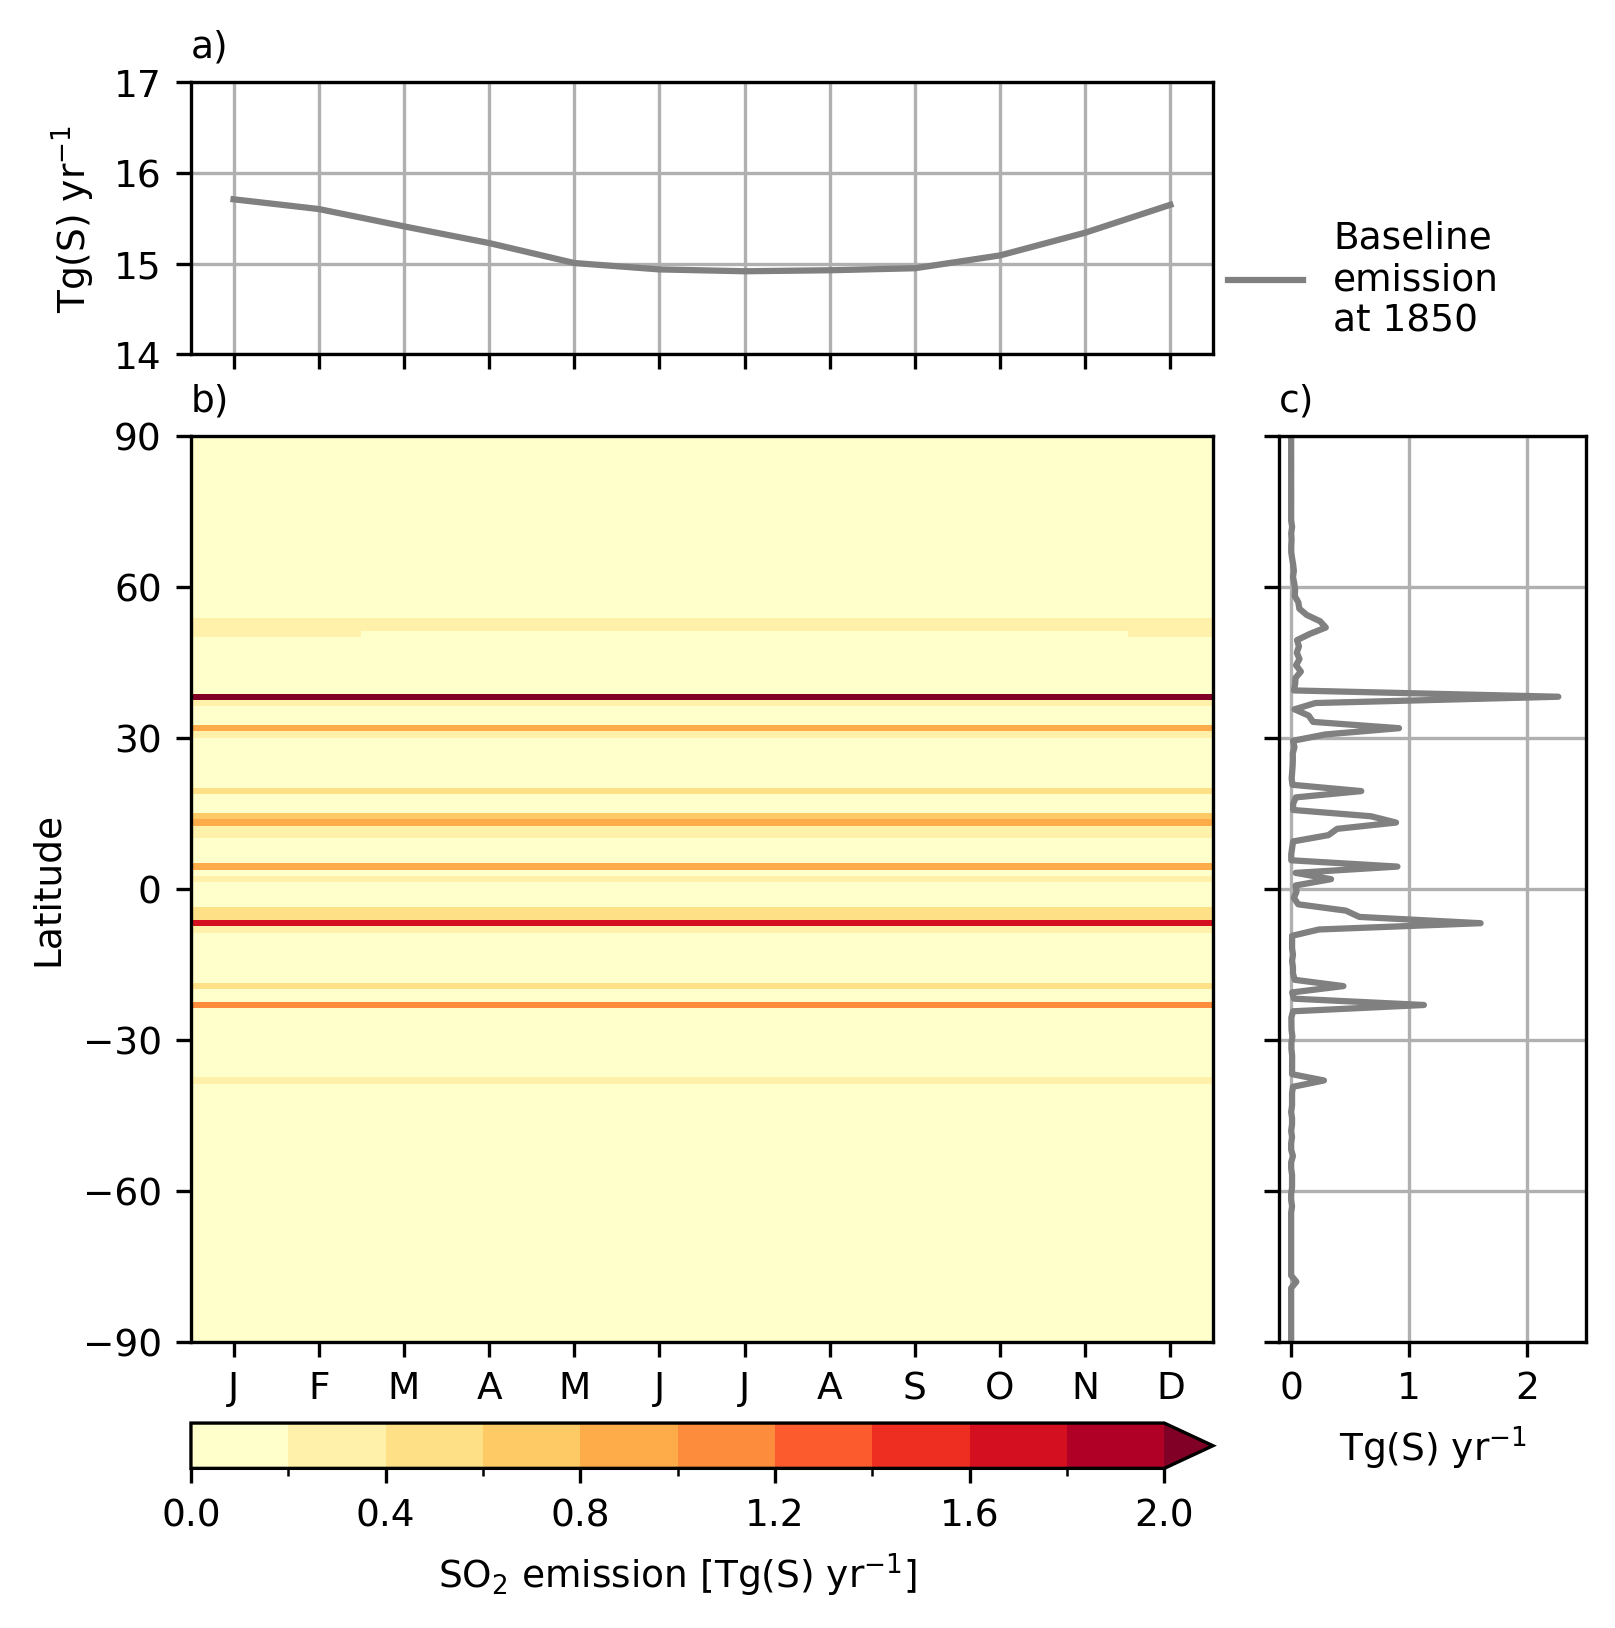
\includegraphics{Appendix1/figs/emiso2_monthly_1850.png}
    \caption{\ce{SO2} emissions at 1850, pre-industrial as used in \piaer{} simulation.}
    \label{fig:app1:seasonal-emiso2-1850}
\end{figure}

\begin{figure}
    \centering
    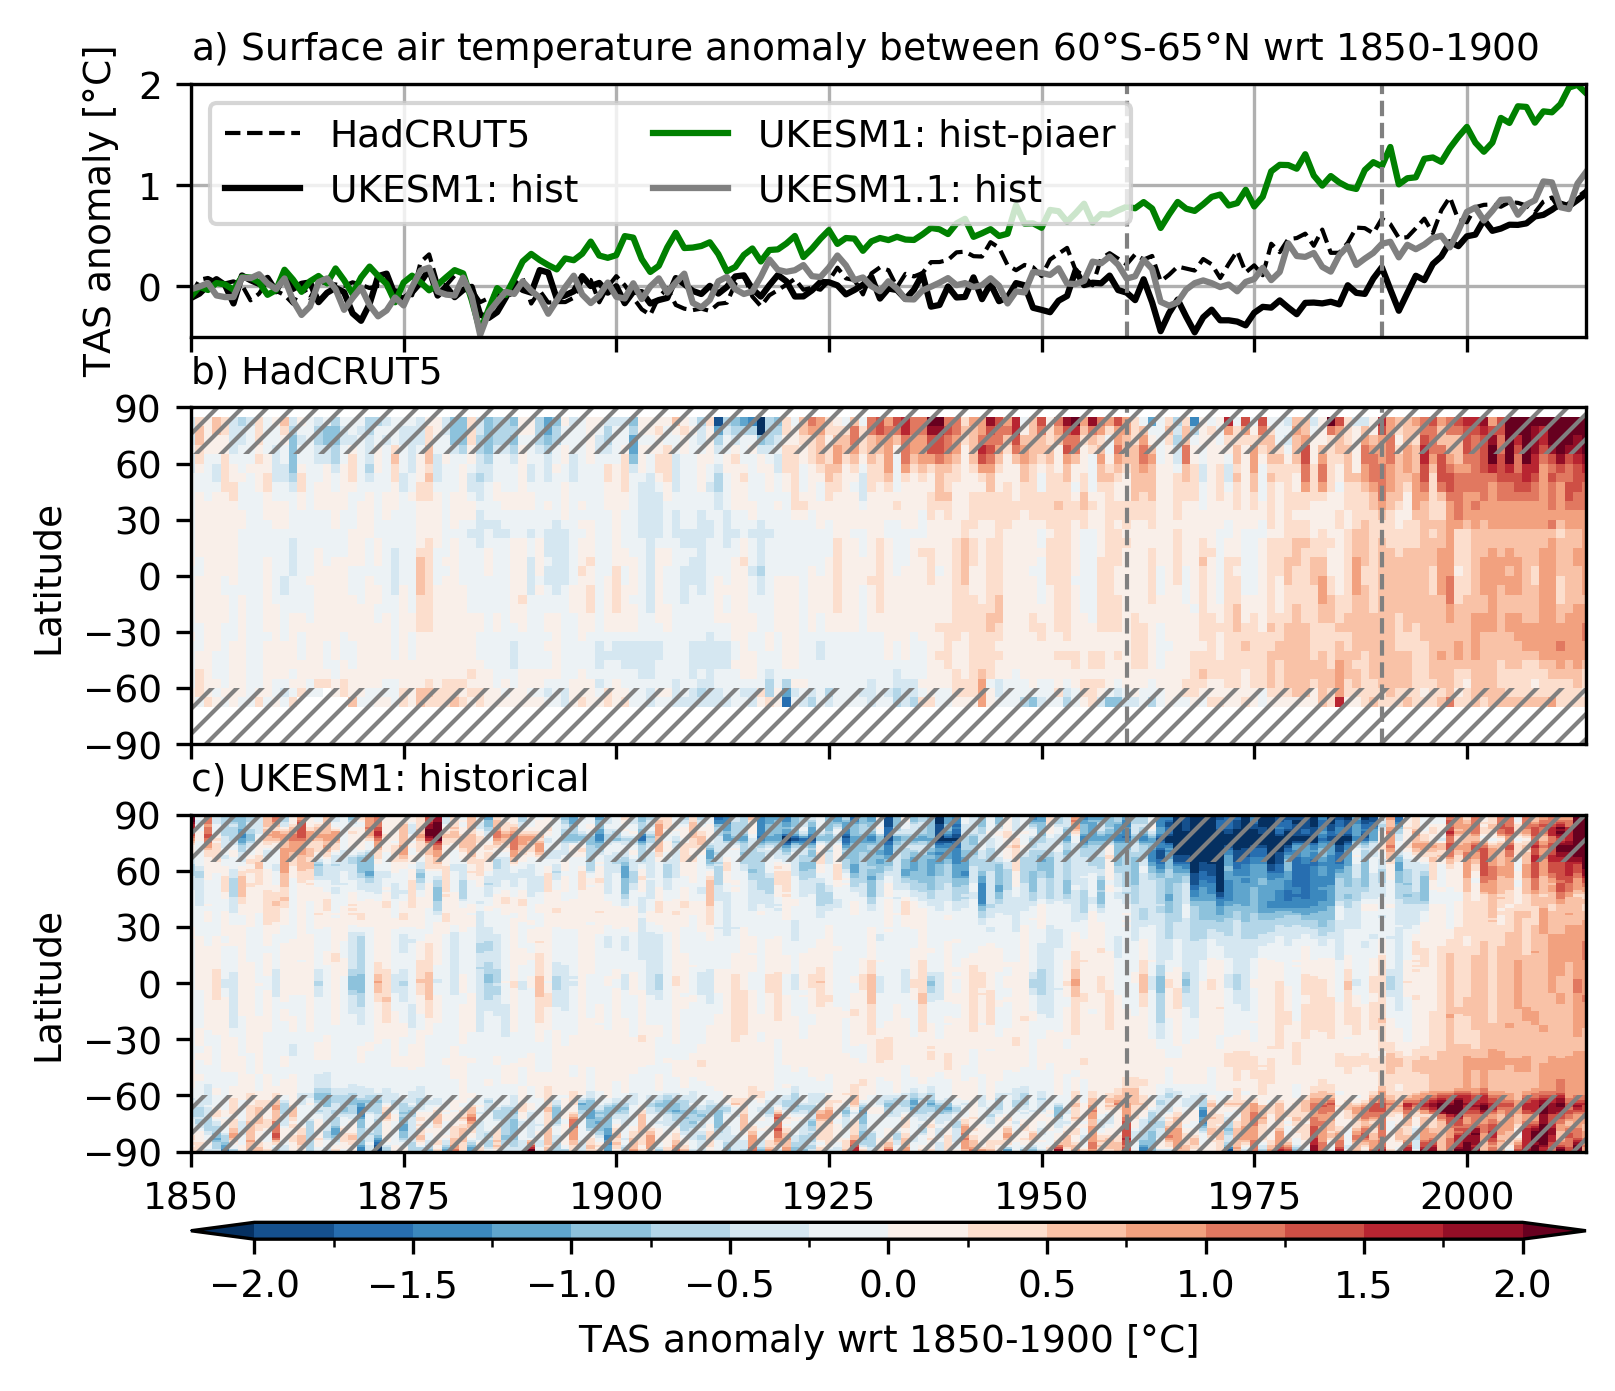
\includegraphics{Appendix1/figs/TAS_anomaly_all.png}
    \caption{Annual mean surface air temperature anomaly between 1850 and 2015 with respect to 1850 and 1900. This plot shows}
    \label{fig:app1:seasonal-emiso2-1850}
\end{figure}

